% Figure F4_tool_states of study_analysis_001 - generated by thesis/study_analysis/figures.py; do not edit by hand.
% Preamble: \usepackage{pgfplots}
%           \pgfplotsset{compat=1.18}
% Analysis tool states (S01/D01, GENERATED - diagnostic)
% Caption: figures/F4_tool_states.caption.tex (figure_caption_tex)
% Composite block, GENERATED (diagnostic only; never mixed with FINAL or STEP rates); S01 (static) / D01 (dynamic) analysis state per tool; COMPLETED does not imply defect-free code; inapplicable states are not analysis gaps
% EFFECTIVE_STATES: Tool states are the effective states (framework.effective_tool_state): a front-end TOOL_ERROR or PARTIAL entry of an artifact whose build failed counts as NOT_ANALYZED (dataset_disclosures.effective_state_overrides); the closure register reports the raw states.
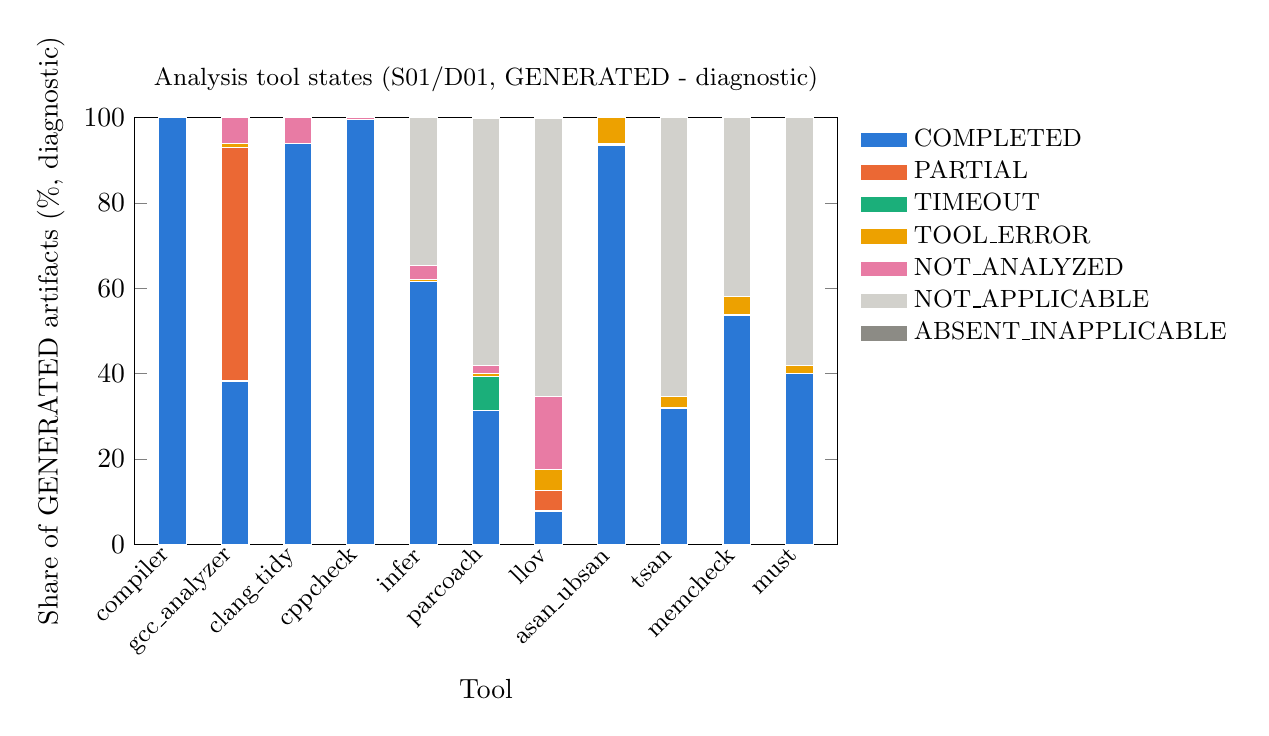
\begin{tikzpicture}
\definecolor{saStateA}{HTML}{2A78D6}
\definecolor{saStateB}{HTML}{EB6834}
\definecolor{saStateC}{HTML}{1BAF7A}
\definecolor{saStateD}{HTML}{EDA100}
\definecolor{saStateE}{HTML}{E87BA4}
\definecolor{saStateF}{HTML}{D2D1CC}
\definecolor{saStateG}{HTML}{8C8B85}
\begin{axis}[
  width=10.5cm,
  height=7cm,
  ybar stacked,
  bar width=10pt,
  ymin=0.000,
  ymax=100.000,
  xtick={0,1,2,3,4,5,6,7,8,9,10},
  xticklabels={{compiler},{gcc\_analyzer},{clang\_tidy},{cppcheck},{infer},{parcoach},{llov},{asan\_ubsan},{tsan},{memcheck},{must}},
  x tick label style={rotate=45,anchor=east,font=\small},
  enlarge x limits=0.06,
  xlabel={Tool},
  ylabel={Share of GENERATED artifacts (\%, diagnostic)},
  legend cell align=left,
  legend style={at={(1.02,1)},anchor=north west,font=\small,draw=none},
  title={Analysis tool states (S01/D01, GENERATED - diagnostic)},
  title style={font=\small}
]
\addplot[fill=saStateA, draw=white, area legend] coordinates {(0,100.000) (1,38.297) (2,94.029) (3,99.524) (4,61.612) (5,31.447) (6,7.821) (7,93.498) (8,31.813) (9,53.736) (10,40.092)};
\addlegendentry{COMPLETED}
\addplot[fill=saStateB, draw=white, area legend] coordinates {(0,0.000) (1,54.725) (2,0.000) (3,0.000) (4,0.000) (5,0.000) (6,4.908) (7,0.000) (8,0.018) (9,0.018) (10,0.000)};
\addlegendentry{PARTIAL}
\addplot[fill=saStateC, draw=white, area legend] coordinates {(0,0.000) (1,0.000) (2,0.000) (3,0.000) (4,0.000) (5,7.839) (6,0.000) (7,0.348) (8,0.128) (9,0.147) (10,0.000)};
\addlegendentry{TIMEOUT}
\addplot[fill=saStateD, draw=white, area legend] coordinates {(0,0.000) (1,0.971) (2,0.000) (3,0.000) (4,0.458) (5,0.806) (6,4.744) (7,6.154) (8,2.619) (9,4.194) (10,1.813)};
\addlegendentry{TOOL\_ERROR}
\addplot[fill=saStateE, draw=white, area legend] coordinates {(0,0.000) (1,6.007) (2,5.971) (3,0.476) (4,3.352) (5,1.813) (6,17.106) (7,0.000) (8,0.000) (9,0.000) (10,0.000)};
\addlegendentry{NOT\_ANALYZED}
\addplot[fill=saStateF, draw=white, area legend] coordinates {(0,0.000) (1,0.000) (2,0.000) (3,0.000) (4,34.579) (5,57.949) (6,65.311) (7,0.000) (8,65.421) (9,41.905) (10,58.095)};
\addlegendentry{NOT\_APPLICABLE}
\addplot[fill=saStateG, draw=white, area legend] coordinates {(0,0.000) (1,0.000) (2,0.000) (3,0.000) (4,0.000) (5,0.147) (6,0.110) (7,0.000) (8,0.000) (9,0.000) (10,0.000)};
\addlegendentry{ABSENT\_INAPPLICABLE}
\end{axis}
\end{tikzpicture}
